\documentclass[fleqn]{jbook}
\usepackage{physpub}

\begin{document}

\begin{question}{専攻 問題1}{}

質量$m$、電荷$e$をもつ一次元の調和振動子がある。時刻$t=0$に一定一様な
電場$F(>0)$が急激に印加されたとき、以下の問に答えよ。ただし、ハミルト
ニアンは
%
\[ H = \left\{\begin{array}{lc}%
         \ds{%
           \frac{p^2}{2m}+\frac{m\omega^2x^2}{2}} & (t<0) \\[3mm]
         \ds{%
           \frac{p^2}{2m}+\frac{m\omega^2x^2}{2}-eFx} & (t \geq 0)
       \end{array}\right. \]
%
であり、$p=-i\hbar\Deriver{}{x}$である。また必要ならば問題末の式を
証明無しに用いてよい。

\begin{subquestions}
\SubQuestion
  $t<0$のハミルトニアンに対応する定常状態について、

  \begin{subsubquestions}
  \SubSubQuestion
    シュレーディンガー方程式を解き、エネルギー固有値$\varepsilon_n$
    と固有関数$\psi_n(x),(n=0,1,2,\cdots)$を求めよ。

  \SubSubQuestion
    横軸を$x$、縦軸をエネルギーとして、ポテンシャルの概形を描き、
    基底状態を含め下から三番目までのエネルギー準位を図中に記入せよ。
    さらに、それぞれの準位に対応した固有関数の概形を描け。

  \end{subsubquestions}

\SubQuestion
  $t\geq 0$のハミルトニアンに対応する定常状態について、

  \begin{subsubquestions}
  \SubSubQuestion
    ポテンシャルの概形を設問{\bf 1}で描いた図中に記入せよ。

  \SubSubQuestion
    シュレーディンガー方程式を解き、エネルギー固有値$E_n$と固有関数
    $\varphi_n(x)\; (n=0,1,2,\cdots)$を求めよ。

  \end{subsubquestions}

\SubQuestion
  $t<0$で基底状態にいた調和振動子の$t \geq 0$での状態・運動を考える。\\
  $t \geq 0$のハミルトニアンのもとで波動関数は、
%
  \[\psi(x,t)=e^{-i\frac{Ht}{\hbar}}\psi(x,0)=\sum_{n=0}^{\infty}
    A_n\varphi_n(x)e^{-i\frac{E_nt}{\hbar}},\;\;\psi(x,0)=\psi_0(x) \]
%
  に従って時間発展する。ここで、 $E_n$は$t \geq 0$でのエネルギー固有値
  、$\varphi_n(x)$は固有関数、$A_n$は$\psi(x,0)$を$\varphi_{n}(x)$で
  展開したときの展開係数である。またこの時の初期状態$\psi(x,0)$は、
  $t<0$での基底状態$\psi_0(x)$である。

  \begin{subsubquestions}
  \SubSubQuestion
    $t \geq 0$で$n$番目の固有状態にいる確率を求めよ。また、この確率は
    どのような確率分布に従うか述べよ。

  \SubSubQuestion
    $t \geq 0$で粒子の存在確率$|\psi(x,t)|^2$が最大の位置
    $x_{\rm max}(t)$はどのように時間発展するか調べよ。また、古典的な
    一次元調和振動子の運動と比較してみよ。

  \end{subsubquestions}
\end{subquestions}

--------------------------------------------------------------------------------------------------------------\\
(参考)エルミート多項式
%
\[ \begin{array}{ll}
     定義 &%
       \ds{ H_n(z) = (-1)^ne^{z^2}%
       \Deriver{^n}{z^n}e^{-z^2} \;\;%
       (n=0,1,2,\cdots)} \\[4mm]
     微分方程式 &%
       \ds{ \left[%
         \Deriver{^2}{z^2}-2z\Deriver{}{z}+2n%
       \right]H_n = 0 } \\[4mm]
     母関数 &
       \ds{ e^{-s^2+2sz} = \sum_{n=0}^{\infty}%
         \frac{s^n}{n!}H_n(z)} \\[4mm]
     直交性 &
       \ds{ \Iint{\d{z}} H_n(z)H_m(z)e^{-z^2}%
       = \sqrt{\pi}2^nn!\delta_{nm}} \end{array}
\]

\end{question}
\begin{answer}{専攻 問題1}{}

\begin{subanswers}
\SubAnswer
  \begin{subsubanswers}
  \SubSubAnswer
    シュレディンガー方程式は
    \[
	\left( \frac{-\hbar^2}{2m}\Partial{^2}{x^2} +
    \frac{m\omega^2x^2}{2} \right) \psi_n(x) = \varepsilon_n \psi_n(x)
    \] 
    長さの次元を持つ量 $\lambda$ を用いて、方程式を無次元化することを
    考える。つまり
%
    \[ \lambda = \sqrt{ \frac{\hbar}{m \omega}}, \hspace{10mm}
       y=x/ \lambda \]
%
    とおいて、シュレーディンガー方程式を書き直す。すると
%
    \[ \left( \Partial{^2}{y^2}-y^2 \right) \psi_n(\lambda y)%
       = - \frac{2\varepsilon_n}{\hbar \omega} \psi_n(\lambda y) \]
%
    となる。この方程式は$y \to \infty $の極限で
%
    \[ \left( \Partial{^2}{y^2}-y^2 \right) \psi_n(\lambda y) = 0 \]
%
    に帰着し、その漸近解は $\psi_n(\lambda y)=e^{\pm y^2/2}$だから、
    ($y \to \infty $の極限で波動関数が発散しないことを要求して)
%
    \[ \psi_n(\lambda y)=e^{-y^2/2} \phi_n(y) \]
%
    とおく。$\psi$についての方程式を$\phi$についての方程式に書き直すと
%
    \[ \phi_n^{\prime \prime}(y) -2y\phi_n^{\prime}(y)
       +\left(\frac{2\varepsilon_n}{\hbar\omega}-1\right)\phi_n(y)=0 \]
%
    これはエルミート多項式の満たす微分方程式だから、ただちに
%
    \[ \phi_n(y)=N_n H_n(y), \hspace{10mm}%
       \varepsilon_n=\hbar\omega\left(n+\frac{1}{2}\right),%
       \hspace{10mm} n=0,1,2,... \]
%
    を得る。つまり
%
    \[ \psi_n(x)=N_n e^{-x^2/2\lambda^2} H_n(x/\lambda), \hspace{10mm}%
       \varepsilon_n=\hbar \omega \left( n+\frac{1}{2} \right) \]
%
    となる。ただし
%
    \[ \lambda = \sqrt{\frac{\hbar}{m \omega }}, \hspace{10mm}%
       \frac{1}{2} m \omega ^2 \lambda ^2%
       = \frac{1}{2} \hbar \omega \quad%
       \mbox{(すなわち零点振動の古典的半径)} \]
%
    $N_n$は規格化条件

    \[ \Iint{\d{x}} \psi_n(x)\psi_n(x)%
       = N_n^2 \Iint{\d{(\lambda y)}} e^{-y^2} H_n(y) H_n(y)%
       = N_n^2 \lambda \sqrt{\pi}\,2^nn! = 1 \]
%
    から、
%
    \[ N_n=(\lambda \sqrt{\pi}\, 2^n n!)^{-1/2} \]


  \SubSubAnswer
    \parbox[t]{72mm}{
    $\lambda=1$で規格化した波動関数は
%
    \begin{eqnarray*}
      \psi_0(x) &=&%
        {\pi}^{-\frac{1}{4}} e^{-x^2/2} \\
      \psi_1(x) &=&%
        {\pi}^{-\frac{1}{4}}\frac{1}{\sqrt{2}} e^{-x^2/2} 2x \\
      \psi_2(x) &=&%
        {\pi}^{-\frac{1}{4}}\frac{1}{\sqrt{8}} e^{-x^2/2}(4x^2-2) \\[3mm]
      \psi_0^{\prime}(x) &=&%
       -{\pi}^{-\frac{1}{4}} e^{-x^2/2} x \\
      \psi_1^{\prime}(x) &=&%
       -{\pi}^{-\frac{1}{4}}\frac{1}{\sqrt{2}}e^{-x^2/2}2(x^2-1) \\
      \psi_2^{\prime}(x) &=&%
       -{\pi}^{-\frac{1}{4}}\frac{1}{\sqrt{8}}e^{-x^2/2}(4x^2-10)x
    \end{eqnarray*}
%
    従って右図のようになる。
    }\parbox[t]{82mm}{\vspace*{-10mm}
    \begin{center}
      \mbox{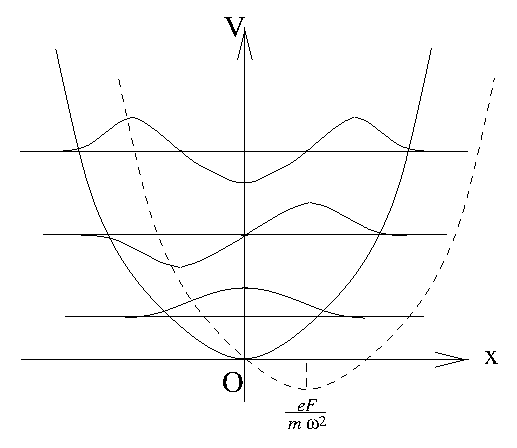
\includegraphics[clip]{1993phy1-1.eps}}
    \end{center}}

  \end{subsubanswers}


\SubAnswer
  \begin{subsubanswers}
  \SubSubAnswer
    ポテンシャルは前問の図の点線のようになる。

  \SubSubAnswer
%
    \[ H = -\frac{\hbar^2}{2m} \Partial{^2}{x^2}%
           +\frac{1}{2}m\omega^2\left(x-\frac{eF}{m\omega^2}\right)^2%
           -\frac{1}{2}\frac{e^2 F^2}{m\omega^2} \]
%
    電場のかかったポテンシャルのつりあいの位置
    $x_0=\frac{eF}{m\omega^2}$を座標原点に、
    $\varepsilon = -\frac{1}{2} \frac{e^2 F^2}{m \omega ^2}%
    = -\frac{1}{2} m \omega^2 x_o^2$ をエネルギー原点とすると 
    設問{\bf 1}と同じになる。従って
%
    \[ \xi=x-x_0 \]
    \[ \varepsilon_n=E_n-\varepsilon \]
%
    とおくことにより{\bf 1}(i)の場合と同様に解ける。答えは
%
    \[ \varphi_n(x) = N_n e^{-\xi^2/2\lambda^2}H_n(\xi/\lambda)%
       \hspace{15mm}%
       \xi=x-x_0,\quad x_0 = \frac{eF}{m\omega^2}, \quad%
       \lambda=\sqrt{\frac{\hbar}{m\omega}} \]

    \[ N_n=(\lambda \sqrt{\pi} 2^n n!)^{-1/2}%
       \hspace{15mm}%
       E_n=\hbar \omega \left( n+\frac{1}{2} \right)+\varepsilon, \quad%
       \varepsilon = -\frac{1}{2} \frac{e^2 F^2}{m \omega ^2}%
       \hspace{15mm}%
       n=0,1,2,... \]
%
    となる。

  \end{subsubanswers}

\SubAnswer
  \begin{subsubanswers}
  \SubSubAnswer
    $\varphi_n(x)$の直交性から、
%
    \begin{eqnarray*}
      A_n%
        &=& \Iint{\d{x}} \varphi_n(x) \psi(x,t=0) %
         = \Iint{\d{x}} \varphi_n(x) \psi_0(x) \\ 
        &=& N_0 N_n \Iint{\d{x}}e^{-\frac{\xi^2}{2\lambda^2}}%
            e^{-\frac{x^2}{2\lambda^2}}H_n(\xi/\lambda) H_0(x/\lambda)
    \end{eqnarray*}
%
    ここで
%
    \[ z = \frac{\xi}{\lambda}, \quad%
       \frac{eF}{\lambda m \omega^2}=\alpha \quad%
       (\lambda で規格化したつりあいの位置 ) \]
%
    と定義すると、
%
    \begin{eqnarray*}
      A_n%
        &=& N_0 N_n \Iint{\d{z}}%
            e^{-\frac{z^2}{2}} e^{-\frac{(z+\alpha)^2}{2}}%
            H_n(z) H_0(z + \alpha) \lambda \\
        &=& N_0 N_n \Iint{\d{z}}%
            e^{-\frac{\alpha^2}{4}} e^{-(\frac{\alpha}{2})^2-z\alpha}%
            e^{-z^2} H_n(z) H_0(z+\alpha) \lambda \\
      \lefteqn{H_0(z)=1を考慮すると}\\
        &=& N_0 N_n \Iint{\d{z}}%
            e^{-\frac{\alpha^2}{4}} e^{-(\frac{\alpha}{2})^2-z\alpha}%
            e^{-z^2}H_n(z) \lambda
    \end{eqnarray*}
%
    また、エルミート多項式の母関数から、$s=-\frac{\alpha}{2}$とすれば、
%
    \[ \exp{(-(\frac{\alpha}{2})^2 - z\alpha)}%
%       = \sum^{\infty}_{n=0}\frac{(\frac{\alpha}{2})^n}{n!} H_n(-z)%
%       = \sum^{\infty}_{n=0}\frac{(\frac{\alpha}{2})^n}{n!}(-1)^n H_n(z)%
       = \sum^{\infty}_{n=0}\frac{(-\frac{\alpha}{2})^n}{n!} H_n(z)%
    \]
%
    これを上の式に代入すると、
%
    \begin{eqnarray*}
      A_n &=& N_0 N_n \Iint{\d{z}} e^{-\frac{\alpha ^2}{4}}%
              \sum^{\infty}_{k=0} \frac{(-\frac{\alpha}{2})^k}{k!}%
              H_k(z) e^{-z^2} H_n(z) \lambda \\
          &=& N_0 N_n \sum^{\infty}_{k=0} \Iint{\d{z}}%
              e^{-\frac{\alpha^2}{4}}\frac{(-\frac{\alpha}{2})^k}{k!}%
              H_k(z) e^{-z^2} H_n(z) \lambda \\
          &=& N_0 N_n \sum^{\infty}_{k=0} e^{-\frac{\alpha^2}{4}}%
              \frac{(-\frac{\alpha}{2})^k}{k!}\sqrt{\pi}2^k k!%
              \delta_{nk} \lambda \\
          &=& N_0 N_n e^{-\frac{\alpha^2}{4}}%
              \frac{(-\frac{\alpha}{2})^n}{n!}\sqrt{\pi}2^nn!\lambda \\
          &=& e^{-\frac{\alpha^2}{4}}(-\alpha)^n%
              \frac{1}{\sqrt{2^n n!}}
    \end{eqnarray*}
%
    つまり
%
    \[ |A_n e^{-i\frac{E_n}{\hbar}t}|^2%
        = |A_n|^2%
        = e^{-\frac{\alpha^2}{2}}(-\alpha)^{2n} \frac{1}{2^n n!}%
        = e^{-\frac{\alpha ^2}{2}}(\frac{\alpha^2}{2})^n \frac{1}{n!}%
    \]
%
    すなわち任意の時刻で系のエネルギーを測定するとエネルギー観測値の
    分布はポアソン分布となる。ただし
%
    \[ \alpha  = \frac{eF}{\lambda m \omega ^2}, \hspace{10mm}%
       \lambda = \sqrt{\frac{\hbar}{m\omega}} \]
%

  \SubSubAnswer
    {\bf 3}(i),{\bf 2}(ii)の結果から、
%
    \begin{eqnarray*}
      \psi(x,t)%
        &=& \sum_ne^{-\frac{\alpha^2}{4}}(-\alpha)^n \frac{1}{2^nn!}%
            \frac{1}{\sqrt{\lambda\sqrt{\pi}}}%
            e^{-\frac{\xi^2}{2\lambda^2}}H_n\left(z\right)
            e^{-i\omega(n+\frac{1}{2})t -i\frac{\varepsilon}{\hbar} t} \\
        &=& e^{-\frac{i\omega t}{2}-i\frac{\varepsilon}{\hbar}t}%
            e^{-\frac{\alpha^2}{4}}\frac{1}{\sqrt{\lambda\sqrt{\pi}}}%
            e^{-\frac{z^2}{2}}%
            \sum_n\left(\frac{-\alpha}{2}e^{-i\omega t}\right)^n%
            \frac{1}{n!}H_n\left(z\right) \\
    \lefteqn{エルミート多項式の母関数より、}\\
        &=& e^{-\frac{i\omega t}{2}-i\frac{\varepsilon}{\hbar}t}%
            e^{-\frac{\alpha^2}{4}}\frac{1}{\sqrt{\lambda\sqrt{\pi}}}%
            e^{-\frac{z^2}{2}}%
            \exp\left(-\frac{\alpha^2}{4}e^{-2i\omega t} 
              -\alpha e^{-i\omega t} z\right)
    \end{eqnarray*}
%
    よって、$|\psi(x,t)|^2$は、
%
    \begin{eqnarray*}
      |\psi(x,t)|^2%
         &=& e^{-\frac{\alpha^2}{2}}\frac{1}{\lambda\sqrt{\pi}}%
             e^{-z^2}\exp\left(\frac{-\alpha^2}{2}%
             \cos2\omega t -\alpha 2z\cos\omega t\right) \\
         &=& \frac{1}{\lambda\sqrt{\pi}}%
             \exp\left( -( \alpha\cos\omega t + z)^2 \right)\\
    \end{eqnarray*}
%
    すなわち波動関数は中心$z=-\alpha\cos\omega t$のガウス分布となる。
    $x$で表せば
%
    \[ x_{\rm max}(t) = \lambda \alpha (1-\cos\omega t) %
        = \frac{eF}{m \omega ^2} (1-\cos\omega t) \]
%
    これは$t=0$で原点に静止していた古典粒子の$t\geq 0$のときの
    ポテンシャル中における運動と一緒である。

  \end{subsubanswers}
\end{subanswers}
\end{answer}


\end{document}
